\documentclass[11pt]{article}\usepackage[]{graphicx}\usepackage[]{color}
%% maxwidth is the original width if it is less than linewidth
%% otherwise use linewidth (to make sure the graphics do not exceed the margin)
\makeatletter
\def\maxwidth{ %
  \ifdim\Gin@nat@width>\linewidth
    \linewidth
  \else
    \Gin@nat@width
  \fi
}
\makeatother

\definecolor{fgcolor}{rgb}{0.345, 0.345, 0.345}
\newcommand{\hlnum}[1]{\textcolor[rgb]{0.686,0.059,0.569}{#1}}%
\newcommand{\hlstr}[1]{\textcolor[rgb]{0.192,0.494,0.8}{#1}}%
\newcommand{\hlcom}[1]{\textcolor[rgb]{0.678,0.584,0.686}{\textit{#1}}}%
\newcommand{\hlopt}[1]{\textcolor[rgb]{0,0,0}{#1}}%
\newcommand{\hlstd}[1]{\textcolor[rgb]{0.345,0.345,0.345}{#1}}%
\newcommand{\hlkwa}[1]{\textcolor[rgb]{0.161,0.373,0.58}{\textbf{#1}}}%
\newcommand{\hlkwb}[1]{\textcolor[rgb]{0.69,0.353,0.396}{#1}}%
\newcommand{\hlkwc}[1]{\textcolor[rgb]{0.333,0.667,0.333}{#1}}%
\newcommand{\hlkwd}[1]{\textcolor[rgb]{0.737,0.353,0.396}{\textbf{#1}}}%

\usepackage{framed}
\makeatletter
\newenvironment{kframe}{%
 \def\at@end@of@kframe{}%
 \ifinner\ifhmode%
  \def\at@end@of@kframe{\end{minipage}}%
  \begin{minipage}{\columnwidth}%
 \fi\fi%
 \def\FrameCommand##1{\hskip\@totalleftmargin \hskip-\fboxsep
 \colorbox{shadecolor}{##1}\hskip-\fboxsep
     % There is no \\@totalrightmargin, so:
     \hskip-\linewidth \hskip-\@totalleftmargin \hskip\columnwidth}%
 \MakeFramed {\advance\hsize-\width
   \@totalleftmargin\z@ \linewidth\hsize
   \@setminipage}}%
 {\par\unskip\endMakeFramed%
 \at@end@of@kframe}
\makeatother

\definecolor{shadecolor}{rgb}{.97, .97, .97}
\definecolor{messagecolor}{rgb}{0, 0, 0}
\definecolor{warningcolor}{rgb}{1, 0, 1}
\definecolor{errorcolor}{rgb}{1, 0, 0}
\newenvironment{knitrout}{}{} % an empty environment to be redefined in TeX

\usepackage{alltt}
\usepackage{amsmath}
\usepackage{stmaryrd}
\usepackage{bbm}
\usepackage{amsmath}
%\usepackage{mathtools}
\newcount\colveccount
\newcommand*\colvec[1]{
        \global\colveccount#1
        \begin{pmatrix}
        \colvecnext
}
\def\colvecnext#1{
        #1
        \global\advance\colveccount-1
        \ifnum\colveccount>0
                \\
                \expandafter\colvecnext
        \else
                \end{pmatrix}
        \fi
}
\newcommand{\argmin}{\arg\!\min}

\author{Thibault Doutre, Student ID 26980469}
\title{STAT230 HW 1 \\
University of California, Berkeley}
\date{\today}
\IfFileExists{upquote.sty}{\usepackage{upquote}}{}
\begin{document}
\maketitle


\section{Load data} 

\begin{knitrout}
\definecolor{shadecolor}{rgb}{0.969, 0.969, 0.969}\color{fgcolor}\begin{kframe}
\begin{alltt}
\hlkwd{load}\hlstd{(}\hlstr{'family.rda'}\hlstd{)}
\hlkwd{attach}\hlstd{(family)}
\end{alltt}
\end{kframe}
\end{knitrout}

\section{Least Squares Regression Line
 $y = b*x + a$} 
 
\begin{knitrout}
\definecolor{shadecolor}{rgb}{0.969, 0.969, 0.969}\color{fgcolor}\begin{kframe}
\begin{alltt}
\hlstd{b} \hlkwb{=} \hlkwd{sum}\hlstd{((weight}\hlopt{-}\hlkwd{mean}\hlstd{(weight))}\hlopt{*}\hlstd{(height}\hlopt{-}\hlkwd{mean}\hlstd{(height)))}\hlopt{/}
  \hlkwd{sum}\hlstd{((height}\hlopt{-}\hlkwd{mean}\hlstd{(height))}\hlopt{^}\hlnum{2}\hlstd{)}
\hlstd{a} \hlkwb{=} \hlkwd{mean}\hlstd{(weight)} \hlopt{-} \hlstd{b}\hlopt{*}\hlkwd{mean}\hlstd{(height)}

\hlkwd{plot}\hlstd{(height,weight,} \hlkwc{main} \hlstd{=} \hlstr{"Least Squares Regression Line"}\hlstd{)}
\hlkwd{abline}\hlstd{(a,b)}
\end{alltt}
\end{kframe}
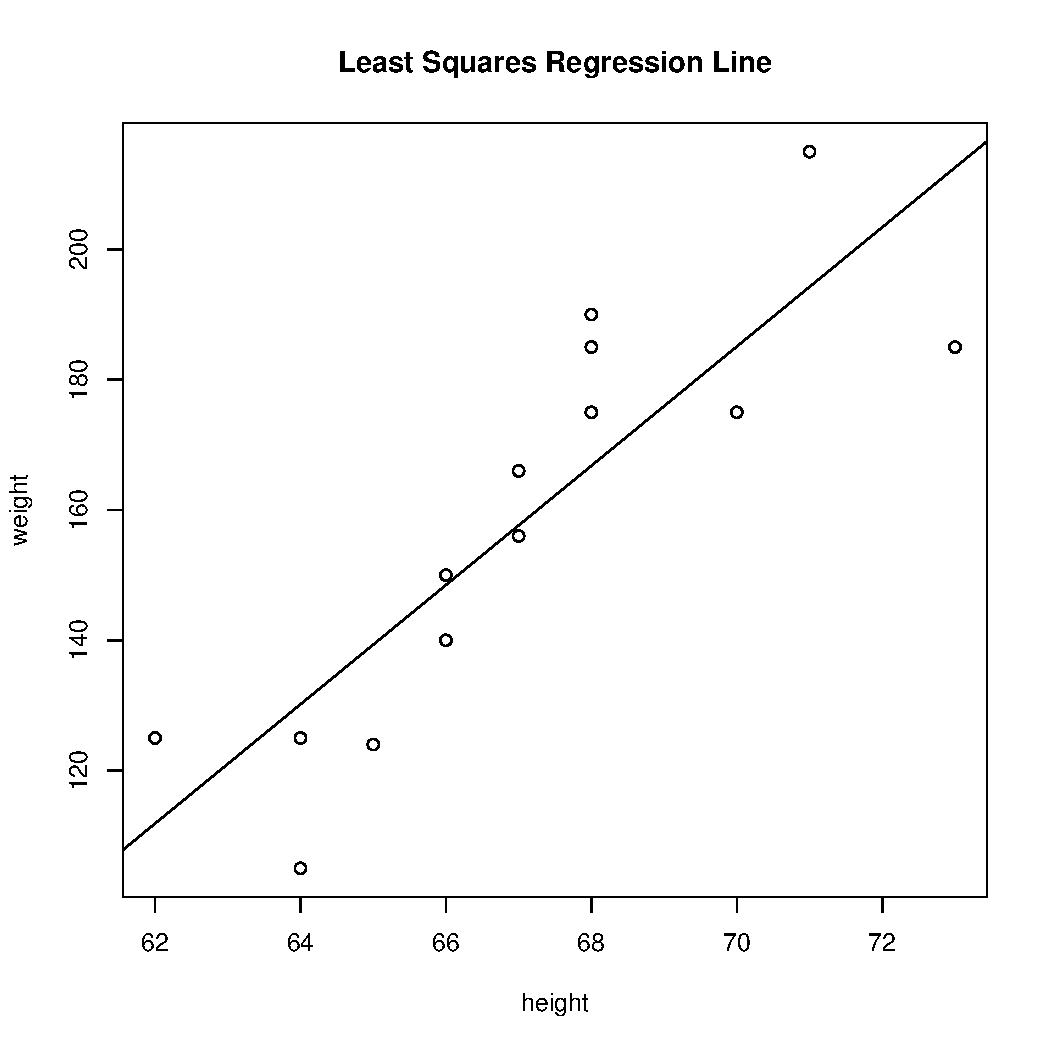
\includegraphics[width=\maxwidth]{figure/unnamed-chunk-2-1} 

\end{knitrout}


\begin{knitrout}
\definecolor{shadecolor}{rgb}{0.969, 0.969, 0.969}\color{fgcolor}\begin{kframe}
\begin{alltt}
\hlstd{regcoef} \hlkwb{=} \hlkwa{function}\hlstd{(}\hlkwc{df}\hlstd{=family[}\hlnum{4}\hlopt{:}\hlnum{5}\hlstd{])\{}
  \hlstd{x} \hlkwb{=} \hlstd{df[,}\hlnum{1}\hlstd{]}
  \hlstd{y} \hlkwb{=} \hlstd{df[,}\hlnum{2}\hlstd{]}
  \hlstd{b} \hlkwb{=} \hlkwd{sum}\hlstd{((y}\hlopt{-}\hlkwd{mean}\hlstd{(y))}\hlopt{*}\hlstd{(x}\hlopt{-}\hlkwd{mean}\hlstd{(x)))}\hlopt{/}\hlkwd{sum}\hlstd{((x}\hlopt{-}\hlkwd{mean}\hlstd{(x))}\hlopt{^}\hlnum{2}\hlstd{)}
  \hlstd{a} \hlkwb{=} \hlkwd{mean}\hlstd{(y)} \hlopt{-} \hlstd{b}\hlopt{*}\hlkwd{mean}\hlstd{(x)}
  \hlkwd{return}\hlstd{(}\hlkwd{c}\hlstd{(a,b))}
\hlstd{\}}

\hlkwd{regcoef}\hlstd{()}
\end{alltt}
\begin{verbatim}
## [1] -455.6660    9.1537
\end{verbatim}
\end{kframe}
\end{knitrout}


\begin{knitrout}
\definecolor{shadecolor}{rgb}{0.969, 0.969, 0.969}\color{fgcolor}\begin{kframe}
\begin{alltt}
\hlstd{regline} \hlkwb{=} \hlkwa{function}\hlstd{(}\hlkwc{df}\hlstd{=family[}\hlnum{4}\hlopt{:}\hlnum{5}\hlstd{])\{}
  \hlstd{coeff} \hlkwb{=} \hlkwd{regcoef}\hlstd{(df)}
  \hlkwd{plot}\hlstd{(height,weight,} \hlkwc{main} \hlstd{=} \hlstr{"Least Squares Regression Line"}\hlstd{)}
  \hlkwd{abline}\hlstd{(coeff[}\hlnum{1}\hlstd{],coeff[}\hlnum{2}\hlstd{])}
\hlstd{\}}

\hlkwd{regline}\hlstd{()}
\end{alltt}
\end{kframe}
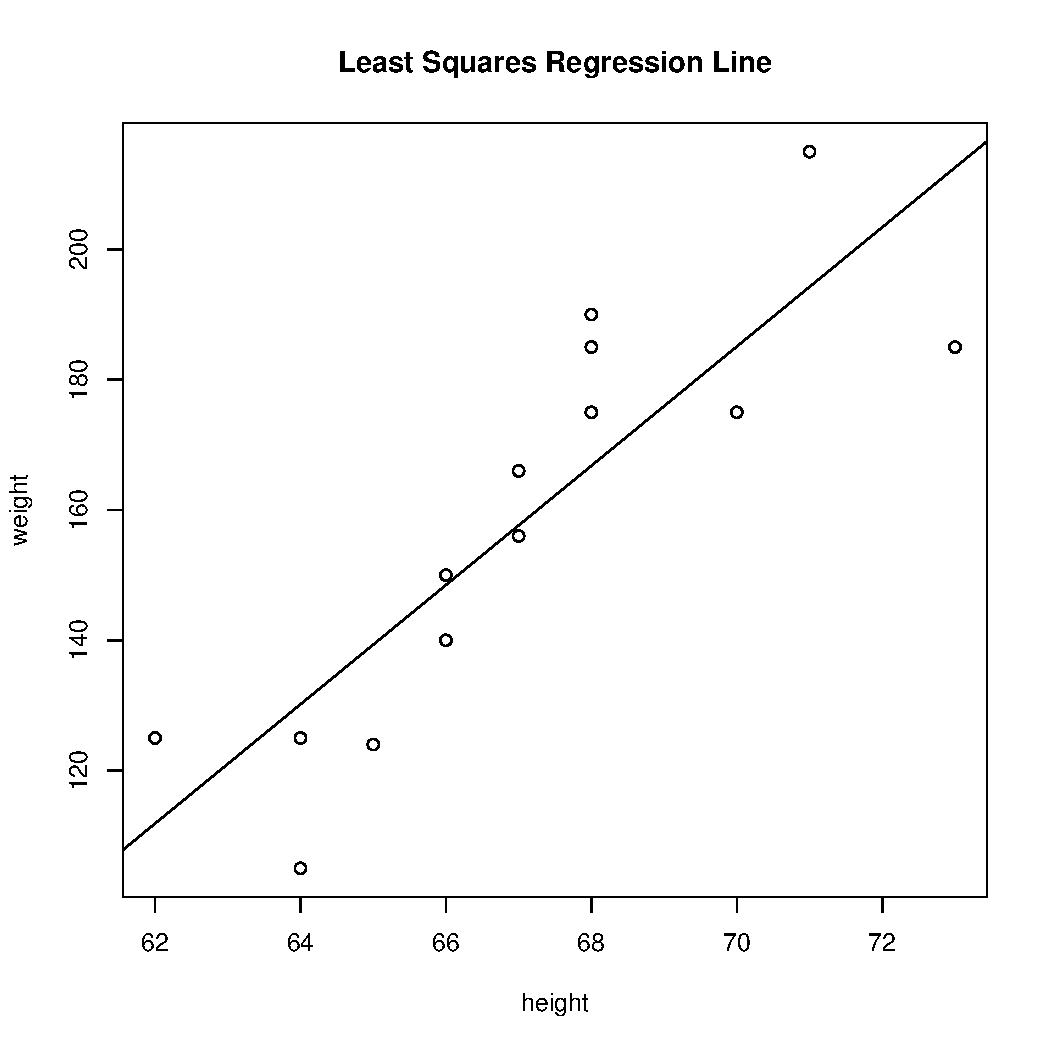
\includegraphics[width=\maxwidth]{figure/unnamed-chunk-4-1} 

\end{knitrout}




\end{document}
